\chapter{Một số phương pháp chung}
\label{ch:methods}

\section{Phương pháp sử dụng bất đẳng thức}

\begin{lythuyetbox}{Sử dụng bất đẳng thức Bunhiacopxki}{mth:bdt-bunhiacopxki}
    \textbf{Bất đẳng thức Bunhiacopxki (Cauchy–Schwarz):}
    
    Với mọi số thực $a_1, a_2, \ldots, a_n$ và $b_1, b_2, \ldots, b_n$, ta luôn có:
    \[
    (a_1^2 + a_2^2 + \cdots + a_n^2)(b_1^2 + b_2^2 + \cdots + b_n^2) \geq (a_1b_1 + a_2b_2 + \cdots + a_nb_n)^2
    \]
    Dấu "=" xảy ra khi và chỉ khi các vector $(a_1, a_2, ..., a_n)$ và $(b_1, b_2, ..., b_n)$ tỉ lệ với nhau.

    \textbf{Trường hợp thường gặp:}
    Với $n=2$, ta có $(a^2+b^2)(x^2+y^2) \geq (ax+by)^2$.
    Một hệ quả quan trọng dùng để đánh giá các biểu thức lượng giác:
    \[
    -\sqrt{a^2+b^2} \leq a\sin x + b\cos x \leq \sqrt{a^2+b^2}
    \]
\end{lythuyetbox}

\section{Phương pháp vẽ bảng biến thiên}

\begin{lythuyetbox}{Vẽ bảng biến thiên để xét tính đơn điệu của hàm số}{mth:bang-bien-thien}
\textbf{Các bước thực hiện:}

\begin{enumerate}
    \item \textbf{Bước 1:} Xét điều kiện xác định của hàm số.
    \item \textbf{Bước 2:} Tính đạo hàm $y'$.
    \item \textbf{Bước 3:} Tìm các điểm tới hạn, gọi chung là các điểm $x_i$.
    \item \textbf{Bước 4:} Sắp xếp các điểm $x_i$ theo thứ tự tăng dần và lập bảng biến thiên, xét dấu $y'$ trên từng khoảng.
\end{enumerate}

\begin{chuy}{Mẹo xét dấu}{cy:meo-bang-bien-thien}
    Có thể dùng máy tính CASIO chức năng giải bất phương trình để xét dấu của đạo hàm một cách nhanh chóng.
\end{chuy}

\textbf{Ví dụ minh họa}

Xét hàm số $y = x^3 - 3x + 2$.

\begin{itemize}
    \item Hàm xác định với mọi $x \in \mathbb{R}$.
    \item Đạo hàm: $y' = 3x^2 - 3 = 3(x-1)(x+1)$.
    \item $y' = 0 \Leftrightarrow x = -1$ hoặc $x = 1$ (hai điểm tới hạn).
    \item Lập bảng biến thiên:
\end{itemize}

\begin{center}
\begin{tikzpicture}
    \tkzTabInit{$x$/1, $y'$/1, $y$/2}{$-\infty$, $-1$, $1$, $+\infty$}
    \tkzTabLine{,+,z,-,z,+}
    \tkzTabVar{+/ $+\infty$, -/ $4$, +/ $0$, -/ $+\infty$}
\end{tikzpicture}
\end{center}

\textbf{Kết luận:} Hàm số đồng biến trên $(-\infty, -1)$ và $(1, +\infty)$, nghịch biến trên $(-1, 1)$. Các điểm cực trị: cực đại tại $x = -1$ (y=4), cực tiểu tại $x = 1$ (y=0).

\end{lythuyetbox}
